\documentclass{article}

\usepackage{graphicx}
\usepackage{tikz}
\usepackage{tikzsymbols}
\usetikzlibrary{calc,patterns,shapes.geometric}
\pagestyle{empty}
\usepackage[margin=0pt]{geometry}
\geometry{papersize={14in,12in}}

\def\centerarc[#1](#2)(#3:#4:#5){\draw[#1] ($(#2)+({#5*cos(#3)},{#5*sin(#3)})$) arc (#3:#4:#5);}

\begin{document}
	\begin{figure}
		\centering
		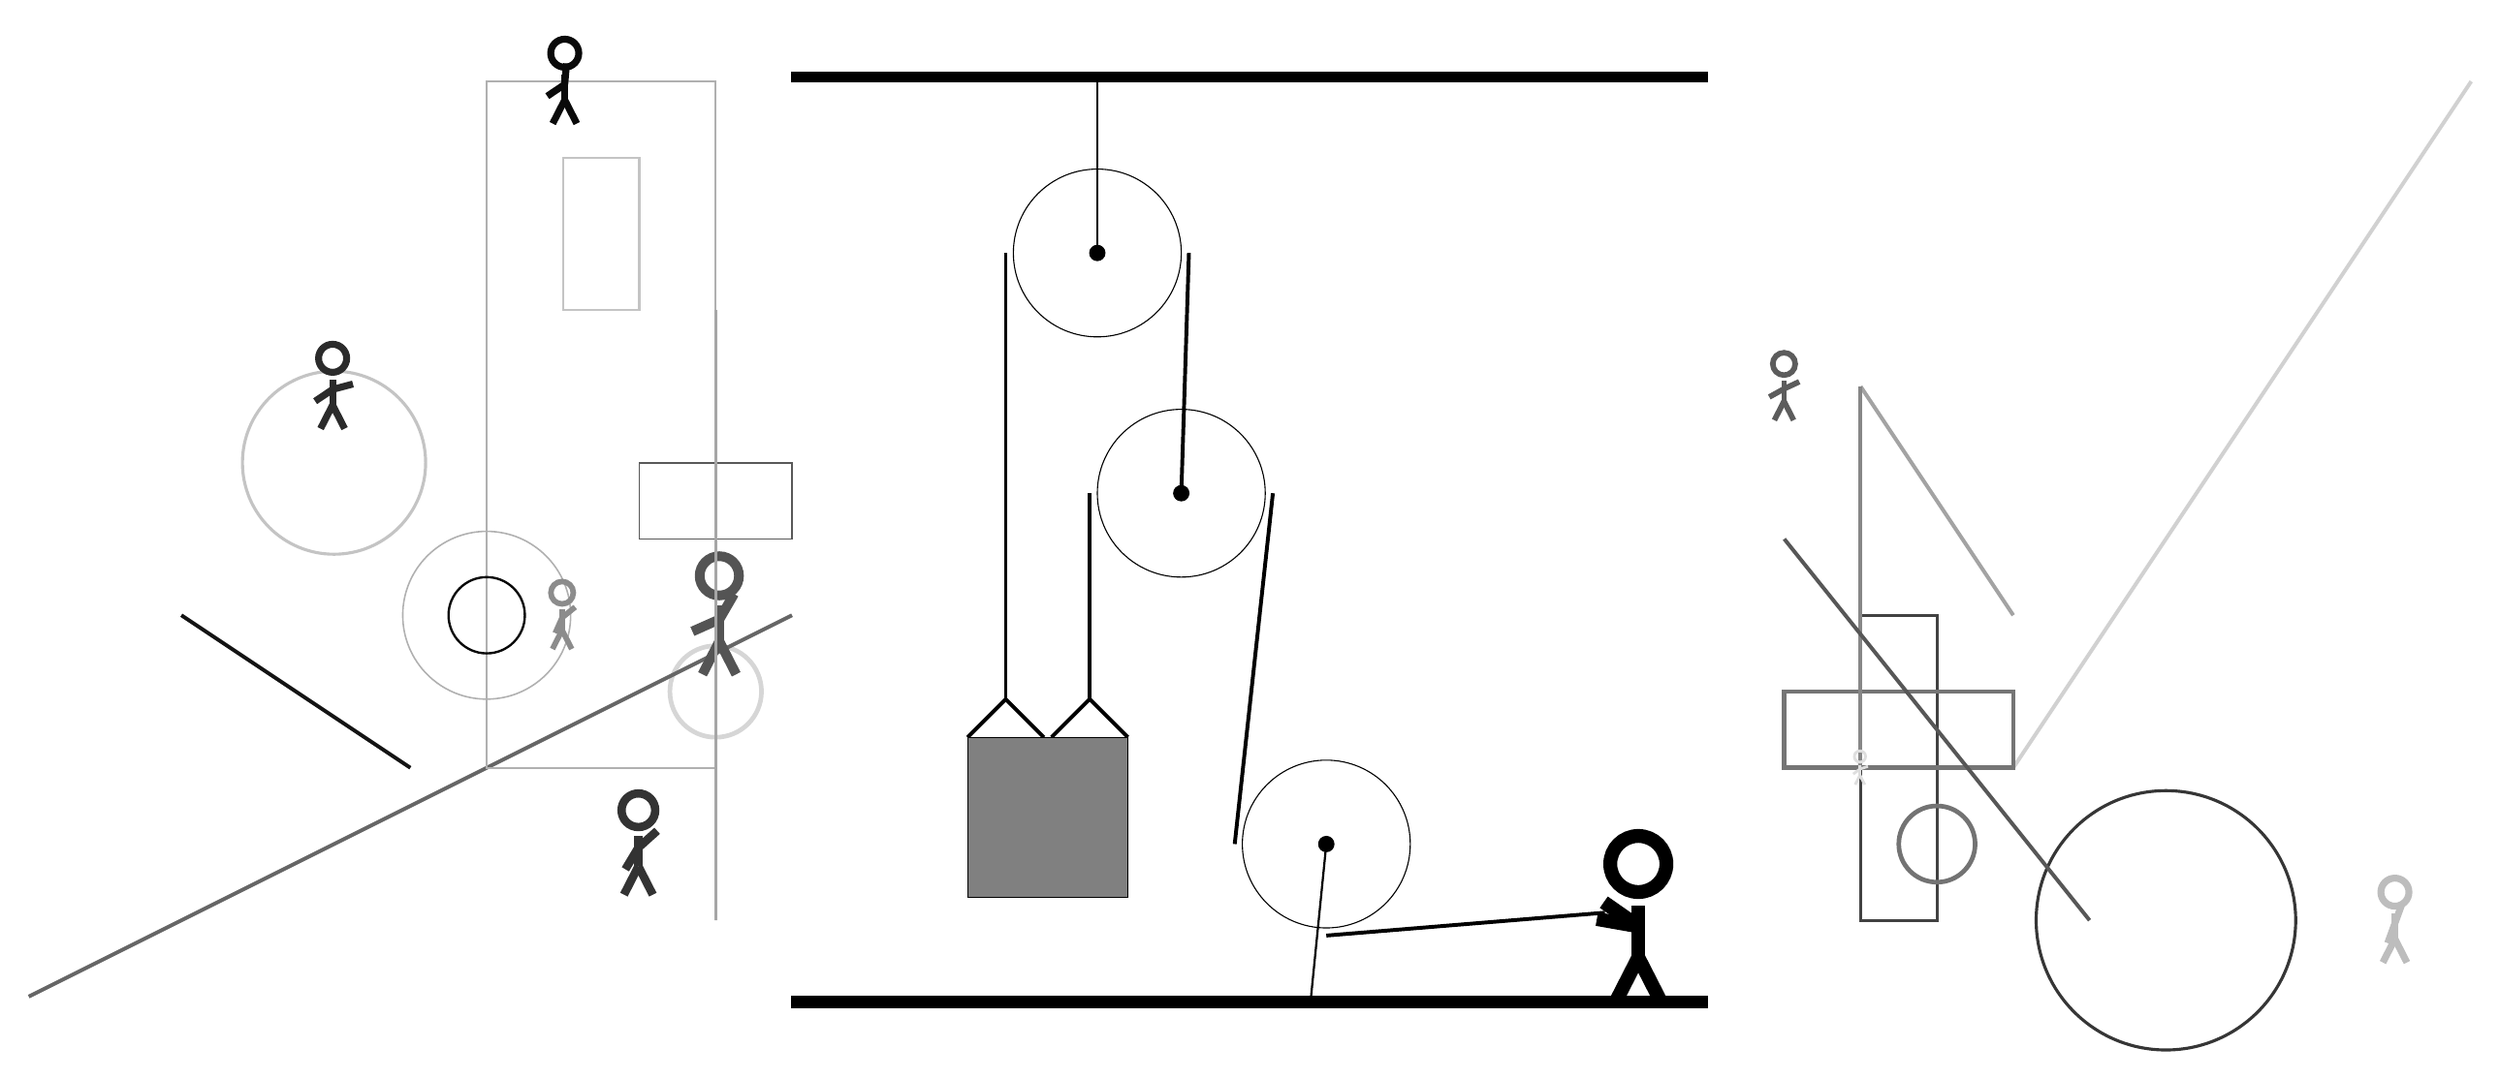
\begin{tikzpicture}
			%%%%% START %%%%%
			
			\draw[fill=black] (-2, 9) rectangle (10, 9.125);
			
			\draw (2, 6.75) circle (1.1);
			\draw[fill=black] (2, 6.75) circle (0.1);
			\draw[thick] (2, 6.75) -- (2, 9);
			
			\draw [line width=0.4mm, color=black!79](16, -2) circle (1.7);
			
			\draw[line width=0.4mm, color=black!74] (12, -2) rectangle (13, 2);
			\draw [line width=0.6mm, color=black!16](-3, 1) circle (0.6);
			\draw[line width=0.5mm, color=black!18](14, 0) -- (20, 9);
			\node[line width=0.7mm, color=black!80] at (-4, -1) {\Strichmaxerl[6][59][42]};
			\draw[line width=0.5mm, color=black!60](-2, 2) -- (-12, -3);
			\node[line width=0.2mm, color=black!67] at (-3, 2) {\Strichmaxerl[7][24][60]};
			\draw[line width=0.6mm, color=black!54] (11, 0) rectangle (14, 1);
			\draw [line width=0.2mm, color=black!31](-6, 2) circle (1.1);
			\draw[line width=0.3mm, color=black!31] (-3, 9) rectangle (-6, 0);
			
			\draw[line width=0.2mm, color=black!65] (-4, 4) rectangle (-2, 3);
			\node[line width=0.7mm, color=black!26] at (19, -2) {\Strichmaxerl[5][70][70]};
			\draw [line width=0.4mm, color=black!23](-8, 4) circle (1.2);
			
			\draw[line width=0.3mm, color=black!23] (-4, 6) rectangle (-5, 8);
			\node[line width=0.3mm, color=black!64] at (11, 5) {\Strichmaxerl[4][29][25]};
			\node[line width=0.2mm, color=black!83] at (-8, 5) {\Strichmaxerl[5][34][15]};
			
			\node[line width=0.3mm, color=black!45] at (-5, 2) {\Strichmaxerl[4][66][39]};
			
			\node[line width=0.2mm, color=black!96] at (-5, 9) {\Strichmaxerl[5][34][85]};
			\draw[line width=0.5mm, color=black!36](14, 2) -- (12, 5);
			\draw[line width=0.5mm, color=black!47](12, 0) -- (12, 5);
			\draw[line width=0.5mm, color=black!66](15, -2) -- (11, 3);
			\draw [line width=0.3mm, color=black!97](-6, 2) circle (0.5);
			\draw [line width=0.6mm, color=black!55](13, -1) circle (0.5);
			\draw[line width=0.5mm, color=black!92](-7, 0) -- (-10, 2);
			\node[line width=0.4mm, color=black!13] at (12, 0) {\Strichmaxerl[2][37][18]};
			
			\draw[line width=0.4mm, color=black!35] (-3, 6) rectangle (-3, -2);
			
			\draw (3.1, 3.6) circle (1.1);
			\draw[fill=black] (3.1, 3.6) circle (0.1);
			
			\draw (5, -1) circle (1.1);
			\draw[fill=black] (5, -1) circle (0.1);
			\draw[thick] (5, -1) -- (4.8, -3);
			
			\draw[line width = 0.5mm]  (0.3, 0.4) -- (0.8, 0.9) -- (1.3, 0.4);
			\draw[line width = 0.5mm]  (1.4, 0.4) -- (1.9, 0.9) -- (2.4, 0.4);
			\draw[fill=black!50] (0.3, 0.4) rectangle (2.4, -1.7);
			
			\draw[line width = 0.5mm] (0.8, 6.75) -- (0.8, 0.9);
			\centerarc[line width = 0.5mm](2, 6.75)(0:180:1.2000000000000002);
			\draw[line width = 0.5mm] (3.2, 6.75) -- (3.1, 3.6);
			\draw[line width = 0.5mm] (1.9, 3.6) -- (1.9, 0.9);
			\centerarc[line width = 0.5mm](3.1, 3.6)(0:180:1.2000000000000002);
			\draw[line width = 0.5mm] (4.3, 3.6) -- (3.8, -1);
			\centerarc[line width = 0.5mm](5, -1)(180:270:1.2000000000000002);
			\draw[line width = 0.5mm] (5, -2.2) -- (8.65, -1.9);
			
			\node at (9, -2) {\Strichmaxerl[10][-35][170]};
			
			\draw[fill=black] (-2, -3) rectangle (10, -3.15);
			
			%%%%% END %%%%%
		\end{tikzpicture}
	\end{figure}	
\end{document}